\documentclass[a4paper, 11pt]{article}
\usepackage{hhline}
\usepackage{amsmath}
\usepackage{amssymb}
\usepackage{graphicx}
\usepackage{mathtools}
\usepackage{color, soul}

% Additional Packages Here
\usepackage[numbers]{natbib}
\usepackage[user, titleref]{zref}
\usepackage{wrapfig}


\graphicspath{{./images/}}

\title{3rd Year Software Engineering Group Project Report}
\author{Group 4 - rh4618, hyk3018, eh4418, yxj18, as16418, dr3818}

\begin{document}
  \maketitle

  \section{Executive Summary}

  \section{Introduction}
    \subsection{Motivation}
      The fashion industry is an important sector of the global economy, contributing up to US\$2.5 trillion in global output.\cite{jec-economic-fashion} The industry is projected to grow, with revenues poised to increase by 8.5\% per annum, and global consumption of apparel to rise from 62 million metric tons in 2019 to 102 million tons in 10 years.\cite{world-bank-enviro} In the past few decades, fast fashion has grown from strength to strength, attracting consumers by offering trendy fashion items for cheap prices. Among some of the most prominent names in this segment include Zara, H\&M and Forever 21, brands that are known for stocking their stores with new items almost weekly, unlike the traditional approach of seasonal releases. \cite{investopedia-fashion} 
      \newline\newline
      Despite the booming financial prospects in this sector, it has created a culture where clothing is disposed of after only having been worn for very few times in favour of new styles in stores, which has in turn ushered in high levels of wastage in the industry, with up to 85\% of textiles produced in a year ending up in landfills. With the invention of polyester fibre in the 1940s, it has become one of the most prevalent fabrics in clothing.\cite{weforum-fashion} However, the material requires large amounts of oil to produce, and can only be broken down into microplastics, which is non-biodegradable and often end up polluting the environment. The production of textiles and fabric is also highly resource-intensive and polluting: each year the industry expends up to 93 billion cubic meters of water.\cite{world-bank-enviro} On the other hand, the fashion industry created up to 2.1 billion tonnes of carbon emissions in 2018, about 4 percent of the global total.\cite{mckinsey-fashion} There is also the aspect of human cost, with many reports of underpaid workers, unsafe work conditions and rampant exploitation particularly associated with fast fashion.\cite{forbes-sweatshops} 
    \subsection{Objective}
      The initial objective of this project is to help users calculate and keep track of their carbon footprint in a convenient way. We decided to focus exclusively on the consumption of clothing as opposed to more commonly addressed areas such as food consumption and transport, encouraging a more sustainable use of clothing items among users. Our application will accompany users through the entire lifecycle of a clothing item from the moment it is purchased up to the moment it is discarded. We aim to inform users of the environmental consequences of their purchase of clothing items in the form of simple numerical metrics that can be tracked and compared. This will also help users understand the environmental impact of different clothing materials and origin, helping them make more informed choices in the future. When a user decides to no longer wear a clothing item, we want to provide suggestions of suitable venues where clothing can be donated instead of being discarded. We hope that the usage of our application improves the user’s awareness of the carbon footprint of their clothing purchases and encourages the user toward sustainable consumption of fashion. 
    \subsection{Primary Achievements}
      The application aims to inform users about the environmental impact of their wardrobe choices, and at the same time bring about a behavioural change by encouraging them to re-wear items in their closet as opposed to buying new clothing items. A scanner used to scan clothing tags which automatically recognises both the material and the place of manufacture of the clothing item to achieve the first goal. We then inform users about the carbon footprint of the clothing item and the number of recommended times the item should be worn to offset the environmental impact. We understand the limitations an informative app have on behavioural change since it might be boring to use hence we decided to add in a closet manager to achieve the second goal. 

  \section{Design and Implementations}
    \begin{figure}[!htbp]
      \centering
      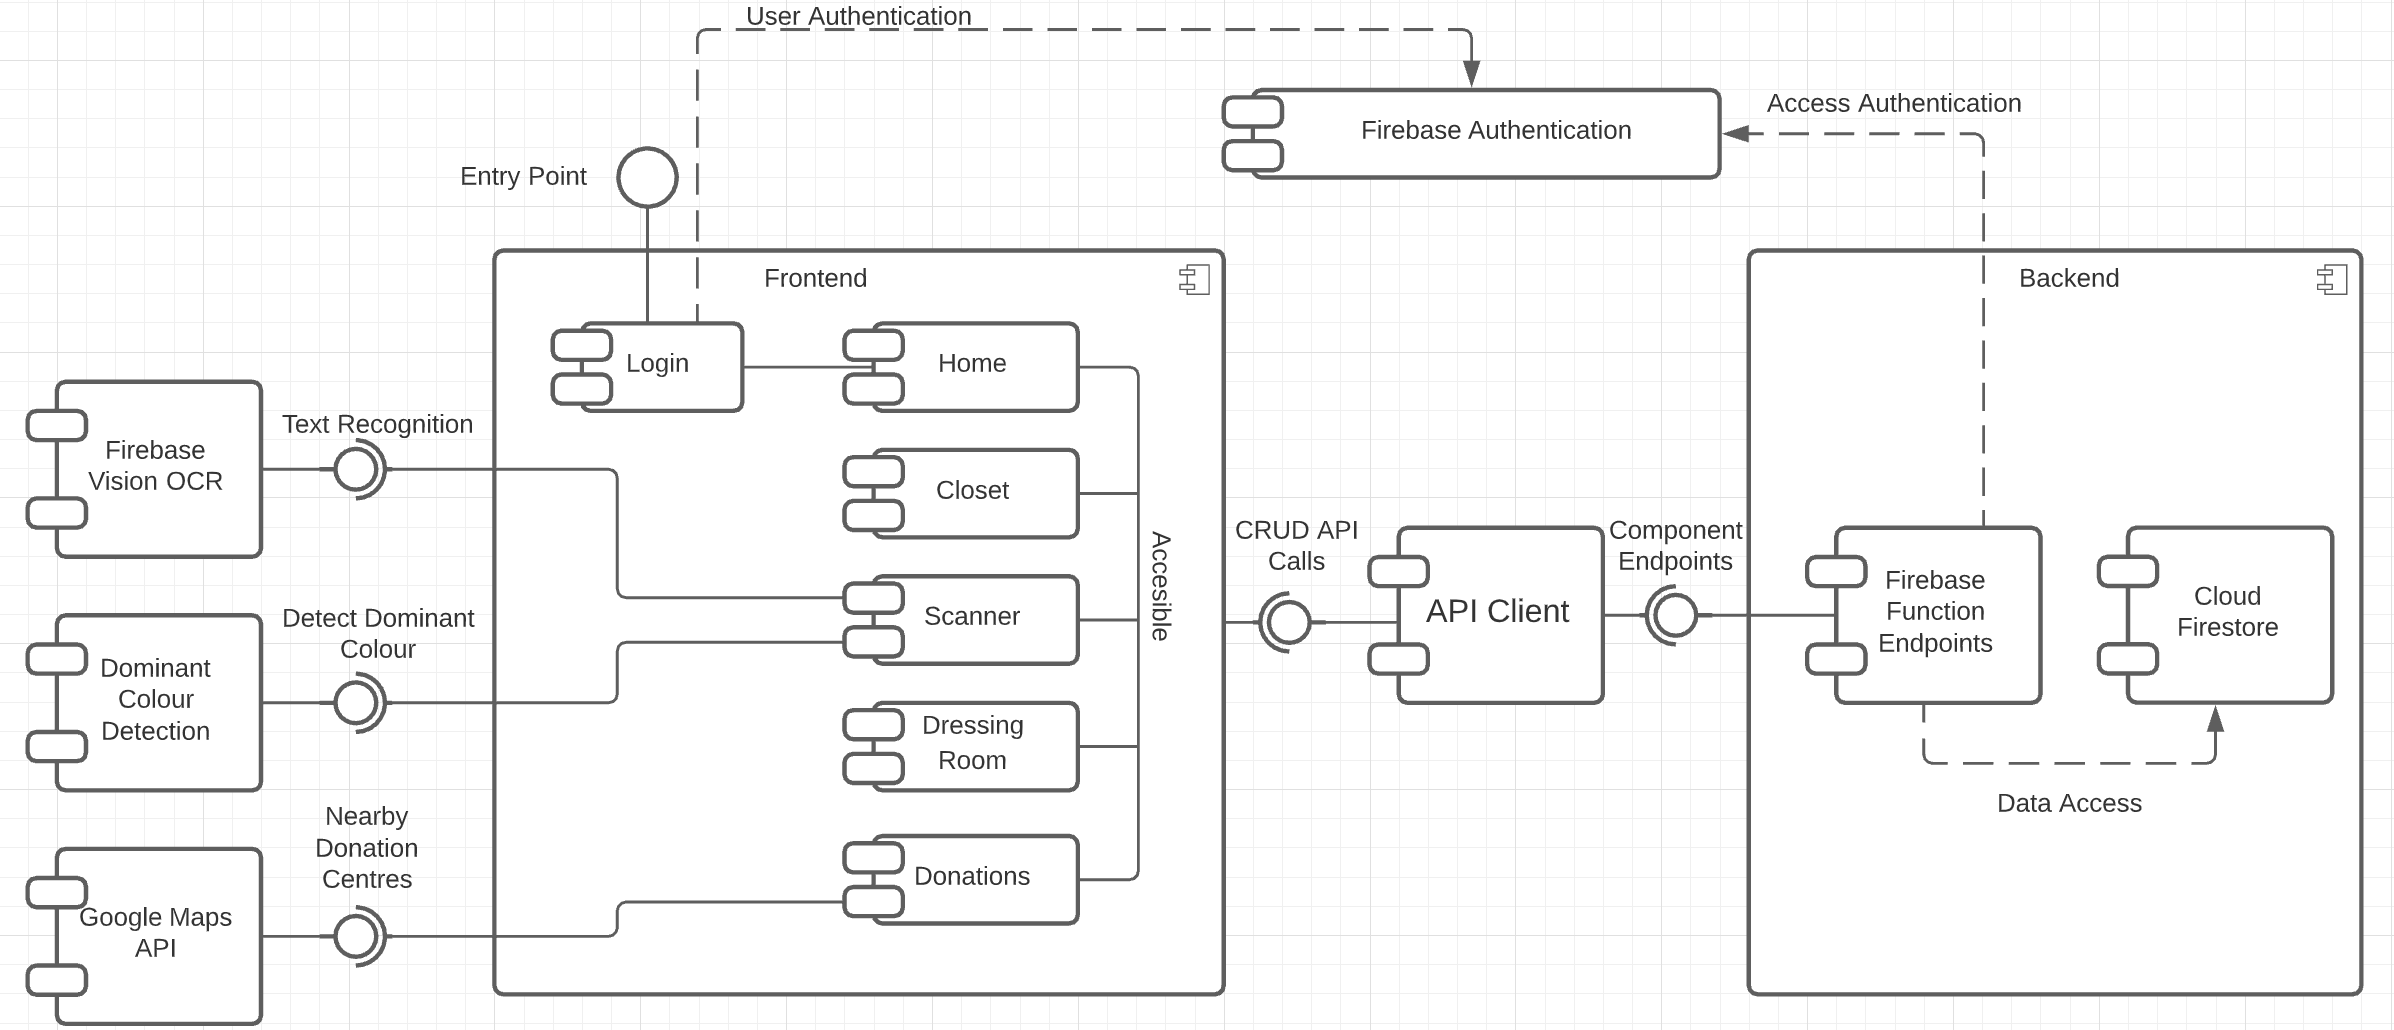
\includegraphics[width=\textwidth]{component-overview.png}
      \caption{UML Diagram of Main Components}
    \end{figure}

    \subsection{Design Overview}
      For ease of implementation and maintenance, we split our functionality
      across different modules, mainly into groups of frontend, backend modules
      as well as the services or APIs used by either of the aforementioned
      groups.
      \newline\newline
      A series of \texttt{Login} pages are the entry points to the program in
      the event that the user has yet to sign in. Once a user has logged in a
      token is saved to the session, which allows for the user to avoid further
      logins so long as the session remains active.
      \newline\newline
      The functionality of the application is accessible from the user starting
      at the \texttt{Home} page, where a summary of the user's progression
      within the application is easily visible. From here, using the navigation
      bar, all other app modules are accessible directly.
      \newline\newline
      The \texttt{Closet} page, where the user could view and manage their added
      items of clothing. The \texttt{Dressing Room} page allows users to create
      and save outfits, which can be worn en masse, to represent items of
      clothing commonly worn together. The \texttt{Donations} page where nearby
      donation centres are located on a map to aid the user to donating their
      items of clothing. The \texttt{Scanner} allows the user to scan in items
      of clothing to their closet, or simply view the carma worth of an item of
      clothing when browsing.
      \newline\newline
      The backend contains the \texttt{Cloud Firestore} database, which stores
      the data required for the running of our application. The \texttt{Firebase
      Function Endpoints} are access components that query the database and
      provides useful services to the frontend.
      \newline\newline
      In order to simplify the access between the frontend and backend, we
      created an \texttt{API Client} component which sits between frontend and
      backend which greatly reduced code redundancy and improved code
      reusability.
      \newline\newline
      For security reasons we chose to use \texttt{Firebase Authentication} to
      maintain an index of existing users in our system and to guard access to
      the application frontend and data access on the backend.
      \newline\newline
      Finally throughout our program we used a variety of external APIs and
      self-made service components to enrich the user experience, more detail
      will be provided in their respective sections in
      `\ztitleref{sec:implementation}' below.


    \subsection{Tech Stack}
    \subsection{Key Implementation Details} \zlabel{sec:implementation}
      \subsubsection{User Carma Record}
       To allow users to keep track of their progress in becoming more eco-friendly with the clothes they wear, we decided to track their Carma points activity, so any action that contributes to Carma is recorded and placed in the following day, month and year record. Different time spans of progress were recorded – a design choice was made here to rather than storing each Carma action, we store the Carma accumulated for the last 7 days for each day, last 12 month for each month, and last 5 years for each year. This way, there is no need to store each Carma “action”, but rather the consequence of it. As a result, storage space is saved and there is no need to process the data very much before retrieval – simply read the accumulated Carma data from the backend.
       \newline\newline
       The data collected per user is displayed to them via the home page through a graph. This is accomplished using \texttt{Flutter Charts}, the standard library for charts and graphs in Flutter.

      
      \subsubsection{User Achievements}
       A way of giving users a sense of satisfaction from their actions is via an achievements system. We have designed this to be easily extendable so that future achievements can be added with ease. Developers simply need to add an achievement entry into the backend \texttt{Firestore}, with an achievement ID, name, achievement type and other relevant information. For the front end, the achievement ID needs to then be mapped to image icons used for display – this is accomplished in the achievement image map service, so that changes only need to be made in one place to take into effect. 
       \newline\newline
       Achievements fall under two categories – a level-based achievement where a certain user value (such as amount of clothes they have donated) is compared against level thresholds to obtain a level; the other achievement type is one-off unlockable achievements, such as creating your first outfit or donating your first item.  
    
    \newpage
      \subsubsection{Home Page}
        \begin{wrapfigure}[16]{L}{0.3\linewidth}
            \centering
            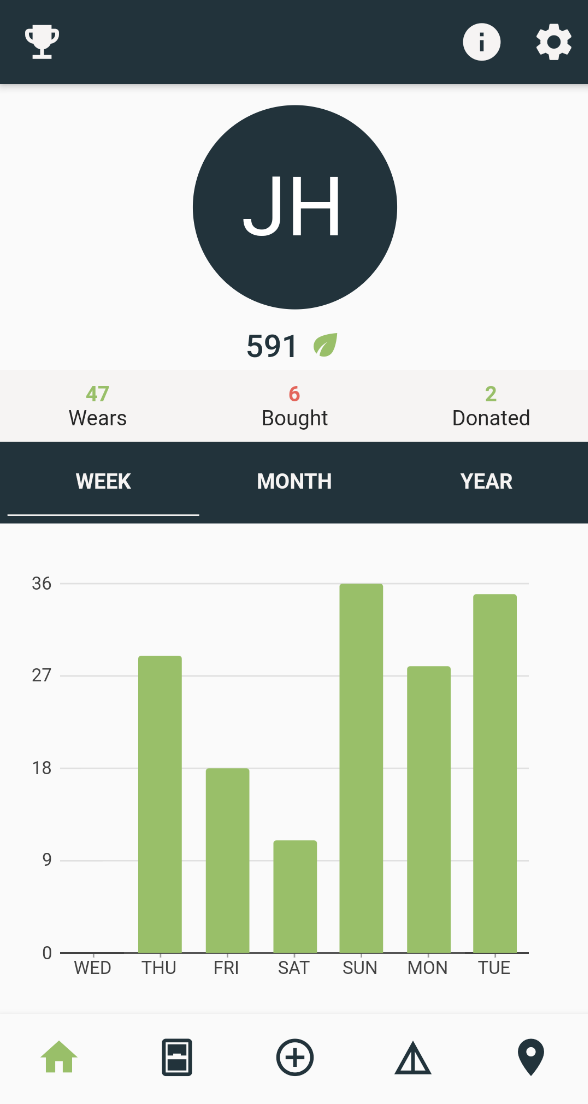
\includegraphics[scale=0.3]{home-page.png}
            \caption{Home Page}
        \end{wrapfigure}
        Our home page serves to display the user's key progression data as they
        use the application. A key part of this is the \texttt{carmaRecord}
        graph, occupying nearly half of the page, which shows the changes to the
        user's total Carma value on a daily basis over the past week, monthly
        basis over the past year or yearly basis over the last 5 years.
        \newline\newline
        Also on this page are records of how many times the user has worn an
        item  of clothing, how many items of clothing does the user own and how
        many items the user has donated. These data records are updated every
        time the app performs a corresponding action such as wearing an item of
        clothing. This is performed on the backend, since update calls through
        the API client assumes data integrity, the frontend does not wait for
        the backend in these instances, thus the performance of the backend in
        updating user records should have minimal visible impact to the user
        experience on the frontend.
        \newline\newline
        Above the Carma records is a value showing the user's total Carma tally,
        as well as the user's avatar. If the user signed in using their google
        account, this space will be populated by their avatar if applicable,
        otherwise we generate an avatar from their initials.
        \newline\newline
        \begin{figure}[!htbp]
          \begin{minipage}[scale=0.45]{0.45\linewidth}
            \centering
            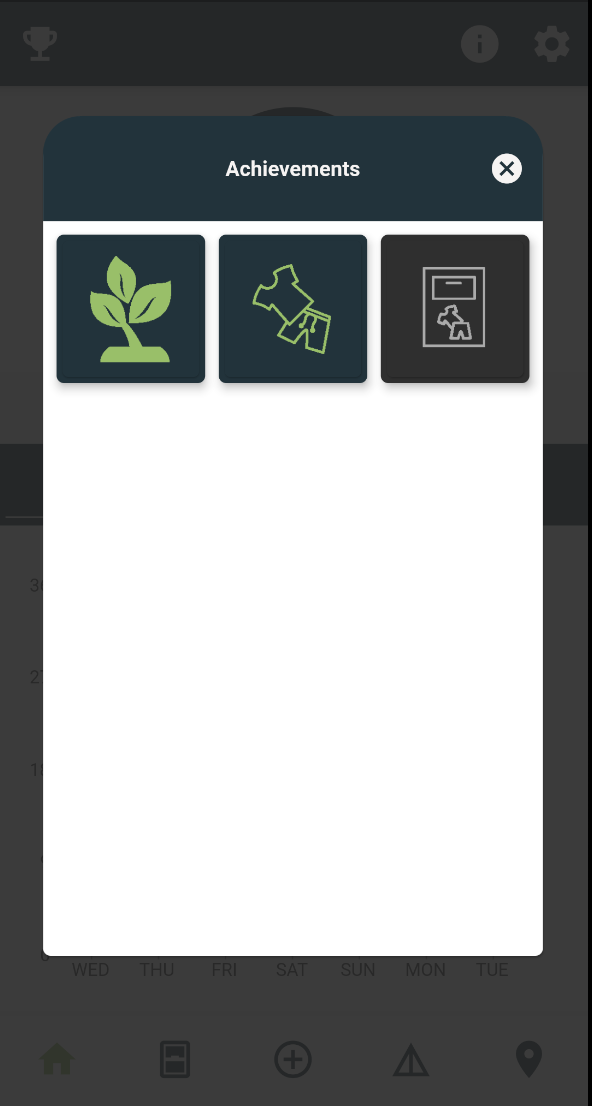
\includegraphics[scale=0.3]{home-achievements.png}
            \caption{Achievement Page}
          \end{minipage}
          \hfill
          \begin{minipage}[scale=0.45]{0.45\linewidth}
            \centering
            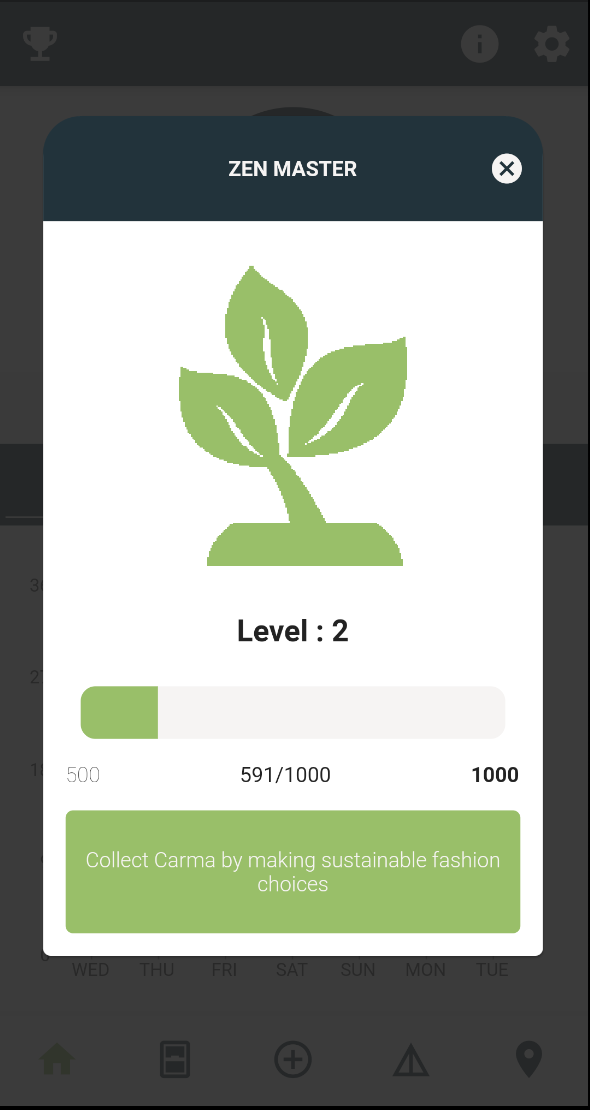
\includegraphics[scale=0.3]{home-achieve-card.png}
            \caption{Achievement Card}
          \end{minipage}
        \end{figure}
        \noindent The achievement button leads to the achievement page where the user can
        view their achievements. Non-achieved one-time achievements are greyed
        out, but the user can still click on the icon to read about the criteria
        and description of each achievement.
        \newline\newline
        The information page is detailed in `\ztitleref{sec:risks}' below.
        \newline\newline
        The additional options button located on the top right is a navigation
        feature, leading to additional functionality such as logout and account
        deletion. The account deletion is a feature added to ensure users are
        given the option to remove their data from our systems at any time.

    \subsection{Technical Challenges}
    \subsection{Risks Encountered and Mitigation} \zlabel{sec:risks}
      For our application, a key point of consideration is the storage and
      security of user data. In an effort to adhere to GDPR principles, there
      were several main areas that we considered.

      \subsubsection{User Photographs}
      Our application requires photographs of user's selected items of clothing
      to be displayed within the user's virtual closet. We have opted for the
      relevant photos to be stored locally on the user's device, as part of the
      application data. This way we do not process nor store the user's
      photographs outside of their device, since we do not control the content
      of the photographs, we could not guarantee that the user photographs did
      not contain information that would be identifiable, and chose to mitigate
      the associated risks thusly.
      \newline\newline
      Storing the user photographs as part of the application data also allows
      for the data to be easily transferred if the user switches device, using
      some form of application cloning tool, which are widespread and easily
      accessible.


      \subsubsection{Storing of User Information for Authentication}
      For the purpose of authenticating a user, we chose to store as little of
      the user's personal information as possible, as most of it did not
      contribute to the user experience of our application. Only the user's
      names are optionally stored within our data storage solution.
      \newline\newline
      We used Firebase Firestore to store our user data, as this allowed for
      custom security rules to our application, which we specified to allow
      access only to users that are authenticated from our Firebase
      Authentication platform\cite{firebase-doc-auth}. In addition to this we
      also enabled users the ability to log in using their google account, which
      further reduced the amount of user personal information that we process.
      So users have the choice to either register an account or to use their
      google account instead, where we only make use of their user avatar and
      display name for our application.
      \newline\newline
      Users also have the option to delete their account at any time, accessible
      as an option via the home screen drawer, whereupon their information will
      be permanently removed from our Firestore and Firebase Authentication
      systems.


      \subsubsection{User Guidance}
      \begin{wrapfigure}[17]{R}{0.3\linewidth}
        \centering
        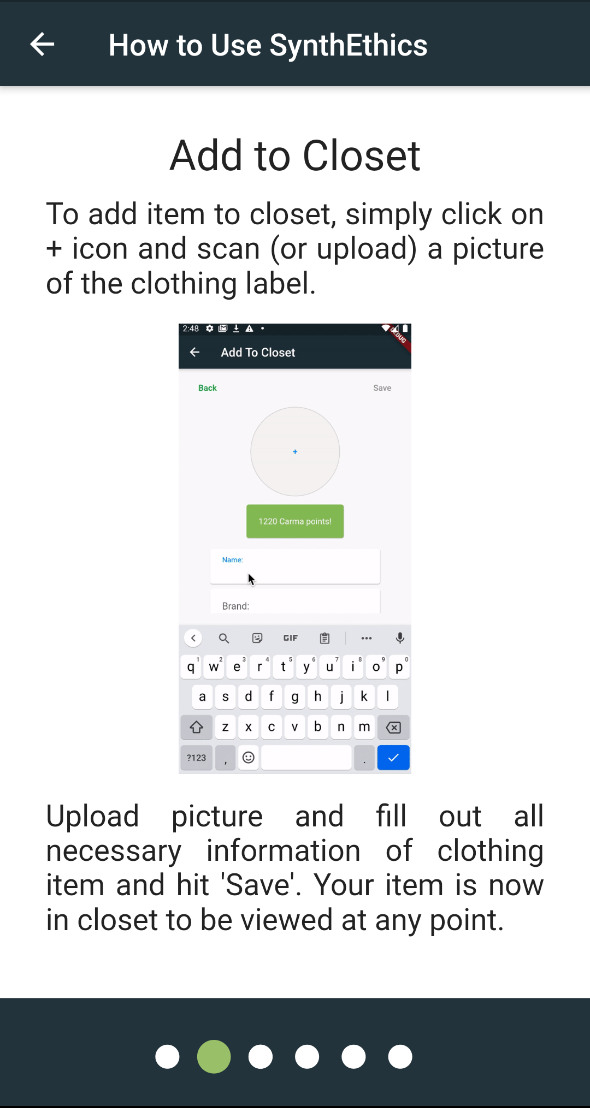
\includegraphics[scale=0.3]{home-info.png}
        \caption{Information Page}
      \end{wrapfigure}
      Throughout our development process we had been actively collecting user
      feedback at regular intervals, a few cases that came up were reports where
      the users were not entirely sure as to how some functionality were
      accessed or the purpose of some buttons. Whilst a majority of our users
      found our UI to be sufficiently intuitive to use, we nonetheless decided
      to facilitate this minority case.
      \newline\newline
      As such from the home page one can press an information button that would
      lead to an information page where the main functionalities of the
      application are described in detail along with gifs demonstrating the use
      of each functionality. We aim for this to inform the user as to how our
      application can be used.

  \section{Evaluation}
    \subsection{Software Quality}
    \subsection{User Evaluation}


  \section{Ethical Considerations}

  \section{Bibliography}
  \bibliographystyle{unsrt}
  \bibliography{bibliography}

  \appendix
  \section{Appendices}



\end{document}